\documentclass{article}
\usepackage[T1]{fontenc}
\usepackage{lmodern}
\usepackage{graphicx}
\usepackage{amsmath,amssymb}
\usepackage[a4paper,margin=2cm]{geometry}
\usepackage[absolute,overlay]{textpos}
\setlength{\TPHorizModule}{1mm}
\setlength{\TPVertModule}{1mm}
\usepackage[indonesian]{babel}
\usepackage{hyperref}
\setlength{\emergencystretch}{2em}
% unit: Halaman 8

\begin{document}

% === Halaman 8 (llm) ===

\vspace{30mm}

Sumber gambar: \textbf{Debdeep Mukhopadhyay, Elliptic Curve Cryptography}, \\
Dept of Computer Sc and Engg IIT Madras

% deskripsi: Kumpulan lima grafik kurva eliptik dengan persamaan yang berbeda: y^2 = x^3 - 1, y^2 = x^3 + 1, y^2 = x^3 - 3x + 3, y^2 = x^3 - 4x, dan y^2 = x^3 - x.
% bbox normalisasi: [0.1800, 0.3000, 0.8300, 0.5600]
\begin{textblock*}{136.50mm}(37.80mm,89.10mm)
\noindent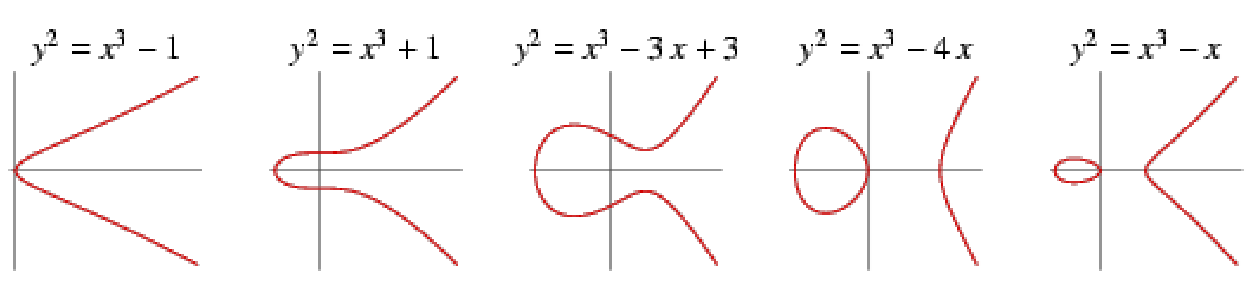
\includegraphics[width=136.50mm,height=77.22mm]{../../images/llm/page_008_img_01.png}%
\end{textblock*}

\end{document}
